\documentclass{beamer}
\usepackage[utf8]{inputenc}
\usepackage[spanish]{babel}
\usepackage{graphicx}
\usepackage{booktabs}
\usepackage{ragged2e}
\usepackage{xcolor}
\definecolor{LightGray}{gray}{0.975}
\definecolor{links}{HTML}{2A1B81}
%\usepackage[urlcolor=blue]{hyperref}
\hypersetup{colorlinks,linkcolor=,urlcolor=blue}

\usepackage{tikz}
\usetikzlibrary{arrows,shapes}

\usepackage{algorithm}
\usepackage{algorithmic}

\usepackage{minted}
\usepackage{xcolor}
\definecolor{LightGray}{gray}{0.975}

\usepackage{listings}

%\usetheme{Warsaw}
\usefonttheme{serif}

\title[DB Security]{Database Administration}
\subtitle{Lecture 08: Database Security.}
\author{Mullins, 2013}
\date{\today}

\setbeamertemplate{navigation symbols}{}%remove navigation symbols

\defbeamertemplate*{footline}{shadow theme}{%
    \leavevmode%
    \hbox{
        \begin{beamercolorbox}[wd=.5\paperwidth,ht=2.5ex,dp=1.125ex,leftskip=.3cm plus1fil,rightskip=.3cm]{author in head/foot}%
            \usebeamerfont{
                author in head/foot
            } Database Administration \hfill \insertshorttitle
        \end{beamercolorbox}%
        \begin{beamercolorbox}[wd=.5\paperwidth,ht=2.5ex,dp=1.125ex,leftskip=.3cm,rightskip=.3cm plus1fil]{title in head/foot}%
            \usebeamerfont{
                title in head/foot
            } \hfill \insertframenumber\,/\,\inserttotalframenumber
        \end{beamercolorbox}
    }
}

\AtBeginSection[]{
    \begin{frame}<beamer>
        \frametitle{Plan}
        \tableofcontents[currentsection]
    \end{frame}
}

\newcommand{\toRight}[1]{
    \begin{FlushRight}
        {\tiny #1}
    \end{FlushRight}
}

\begin{document}

\frame{\titlepage}

\begin{frame}{Database Administration: Database Security.}
    \centering
    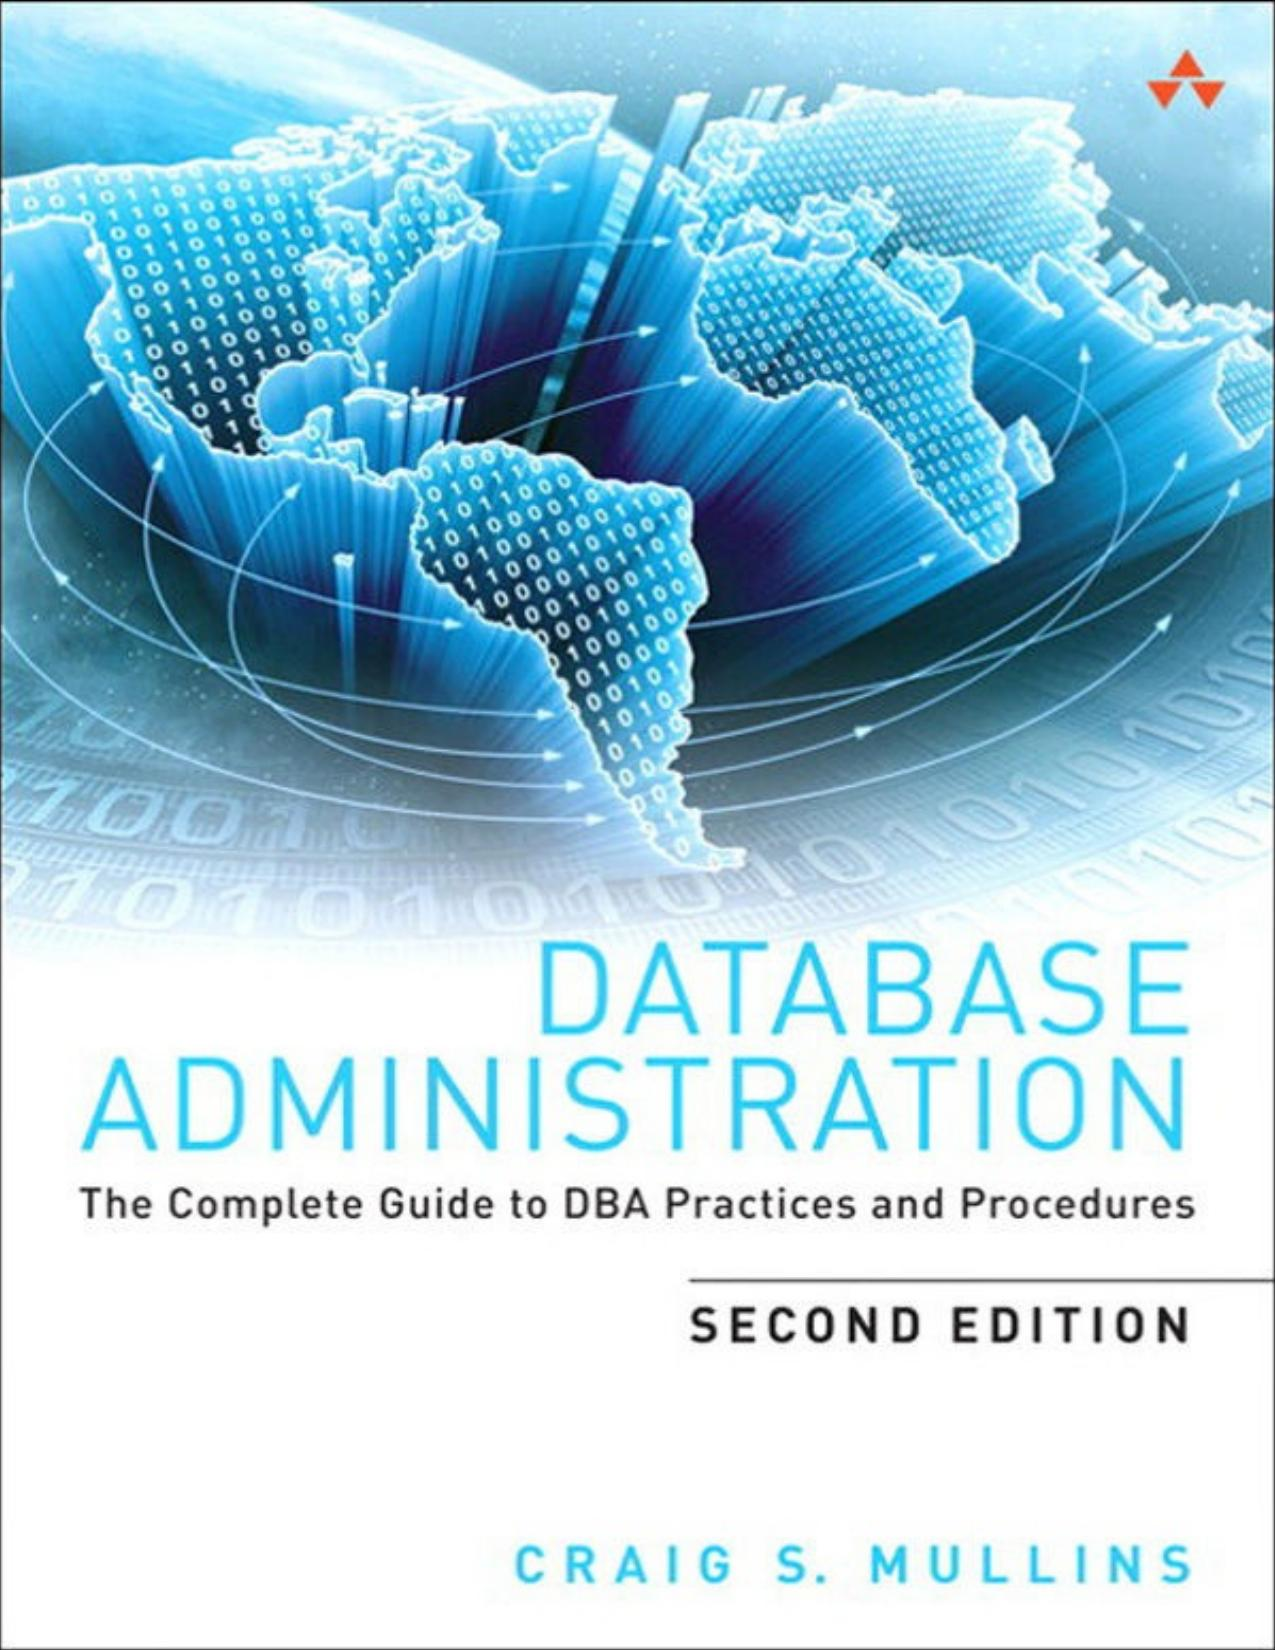
\includegraphics[width=0.4\textwidth]{figures/book_cover}\\
    \vspace{2mm}
    {
        \scriptsize
        Content has been extracted from \textit{Database Administration: The Complete Guide to DBA Practices and Procedure (Chapter 14)}, by Craig Mullins, 2013.  Visit \url{https://www.oreilly.com/library/view/database-administration-the/9780133012743/}.j
    }
\end{frame}

\begin{frame}{Overview}
  \begin{itemize}
    \item Database security is crucial due to increasing data breaches and regulations.
    \item Data breaches are costly and prevalent.
    \item Databases are a prime target for hackers.
    \item Securing data requires a comprehensive plan.
  \end{itemize}
\end{frame}

\begin{frame}{Data Breaches}
  \begin{itemize}
    \item Data breaches continue to rise, with significant impact.
    \item Over 544 million records were breached between 2005 and 2012.
    \item Average cost per lost record is between \$90 and \$305.
    \item Costs include legal fees, customer losses, and bad publicity.
    \item Database servers are the main source of breached data.
  \end{itemize}
\end{frame}

\begin{frame}{Database Security Basics}
  \begin{itemize}
    \item DBMS controls all database resources.
    \item Users must be granted privileges to perform operations.
    \item DBA is typically responsible for database security.
    \item Key aspects of database security:
      \begin{itemize}
        \item Authentication (Who is it?)
        \item Authorization (Who can do it?)
        \item Encryption (Who can see it?)
        \item Audit (Who did it?)
      \end{itemize}
  \end{itemize}
\end{frame}

\begin{frame}{Authentication}
  \begin{itemize}
    \item Strong authentication is essential.
    \item Logins (user IDs) with passwords are required.
    \item Information needed for login creation:
      \begin{itemize}
        \item Password
        \item Default database
        \item Default language
        \item User's full name
        \item Additional details (e.g., email, phone number)
      \end{itemize}
    \item Passwords should be changed regularly.
  \end{itemize}
\end{frame}

\begin{frame}{Password Guidance}
  \begin{itemize}
    \item Passwords should be difficult to guess.
    \item Guidelines:
      \begin{itemize}
        \item Minimum 6 characters, longer if possible.
        \item Use a combination of alphabetic and numeric characters.
        \item Avoid complete words.
        \item Do not embed personal information.
        \item Consider concatenating unrelated words.
        \item Use mnemonic devices, but not obvious ones.
        \item Avoid common and weak password archetypes.
      \end{itemize}
    \item Work with security administration to create and distribute guidelines.
  \end{itemize}
\end{frame}

\begin{frame}{Login Administration}
    \begin{itemize}
        \item Drop logins when no longer needed.
        \item Limit database users who can create database objects to DBAs only.
        \item Lock logins that may need to be reactivated.
        \item Drop logins that will never need to be reactivated.
    \end{itemize}
\end{frame}

\begin{frame}{Database Users}
    \begin{itemize}
        \item Some systems require an additional account to use specific databases.
        \item Login (SUID): Accesses the DBMS or database server.
        \item User name (Database UID): Associated with the login account, required to access each database.
        \item Guest usage can be permitted by configuring a special user name.
    \end{itemize}
    \centering
    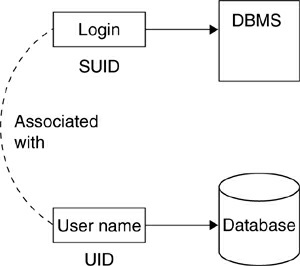
\includegraphics[width=0.3\textwidth]{figures/user_name.png}
\end{frame}

\begin{frame}{Granting and Revoking Authority}
  \begin{itemize}
    \item DBA controls security using Data Control Language (DCL).
    \item DCL statements:
      \begin{itemize}
        \item GRANT: Assigns permission to a database user.
        \item REVOKE: Removes permission from a database user.
      \end{itemize}
    \item GRANT statement requires a list of privileges and users.
    \item WITH GRANT OPTION allows a user to pass the authority to grant privileges.
    \item Avoid issuing GRANT and REVOKE statements from within an application program.
    \item Some DBMSs provide additional functionality (e.g., DENY in SQL Server).
  \end{itemize}
\end{frame}

\begin{frame}{Types of Privileges}
  \begin{itemize}
    \item Basic types: access data, create objects, perform system functions.
    \item Common privilege types:
      \begin{itemize}
        \item Table: Access and modify data within tables.
        \item Database object: Create and drop database objects.
        \item System: Perform system-wide activities.
        \item Program: Create, modify, and use database programs.
        \item Stored procedure: Execute specific functions and stored procedures.
      \end{itemize}
  \end{itemize}
\end{frame}

\begin{frame}{Granting Table Privileges}
  \begin{itemize}
    \item Control access to tables, views, and columns.
    \item Privileges:
      \begin{itemize}
        \item SELECT: Enable user to select from table/view.
        \item INSERT: Enable user to insert rows.
        \item UPDATE: Enable user to update rows/columns.
        \item DELETE: Enable user to delete rows.
        \item ALL: Enable user to select, insert, update, and delete.
      \end{itemize}
    \item Column-level privileges can be specified for SELECT and UPDATE.
\item DBA typically grants table privileges in test environments.
\item Production access should be controlled using program and stored procedure privileges.
\end{itemize}
\end{frame}

\begin{frame}{Granting Database Object Privileges}
    \begin{itemize}
        \item Control permissions to create database structures.
        \item Privileges depend on the DBMS and supported object types.
        \item Options to grant CREATE privileges on various objects (e.g., databases, tablespaces, tables, indexes).
        \item Ability to create objects is usually reserved for DBAs.
        \item Uncontrolled object creation can lead to difficulties in tracking and managing database objects.
    \end{itemize}
\end{frame}

\begin{frame}{Granting System Privileges}
    \begin{itemize}
        \item Control which users can use DBMS features and commands.
        \item Privileges vary from DBMS to DBMS.
        \item Examples: archive logs, shut down/restart server, start traces, manage storage and caches.
        \item System privileges are granted system-wide, not at the database level.
        \item Should be granted with care, usually reserved for DBA and SA.
    \end{itemize}
\end{frame}

\begin{frame}{Granting Program and Procedure Privileges}
    \begin{itemize}
        \item EXECUTE privilege allows users to execute programs or stored procedures.
        \item Granting privileges on programs/procedures is easier to control than on individual tables/columns.
        \item Procedural logic controls which tables and columns can be modified.
        \item DBA can better maintain data integrity by controlling changes programmatically.
    \end{itemize}
\end{frame}

\begin{frame}{Granting to PUBLIC}
    \begin{itemize}
        \item Granting authorization to PUBLIC allows anyone who can log in to the DBMS to have that authority.
        \item Grants to PUBLIC cannot be given with the WITH GRANT OPTION.
        \item Using PUBLIC can appear easier but requires caution.
        \item DBA loses control over the object or resource when a privilege is granted to PUBLIC.
        \item Reserve PUBLIC usage for objects/resources that should be available to everyone.
        \item PUBLIC authority can be a shortcut if another security mechanism is in place (e.g., transaction processor security).
    \end{itemize}
\end{frame}

\begin{frame}{PUBLIC Authority and the System Catalog}
    \begin{itemize}
        \item Dilemma: Whether to grant PUBLIC access to system catalog tables.
        \item Metadata in the system catalog is useful for DBAs, developers, and analysts.
        \item System catalog may contain sensitive information exploitable by hackers (e.g., authorization details, user IDs, login information).
        \item Exposes table names, making it easier for hackers to attempt unauthorized access or SQL injection.
        \item Refrain from granting blanket PUBLIC access to the system catalog tables.
    \end{itemize}
\end{frame}

\begin{frame}{Revoking Privileges}
    \begin{itemize}
        \item REVOKE statement removes previously granted privileges.
        \item Syntax is the "flip side" of the GRANT syntax.
        \item Privileges are automatically revoked when a database object is dropped.
        \item Revoking a PUBLIC privilege does not remove it from users granted it in a separate GRANT statement.
    \end{itemize}
\end{frame}

\begin{frame}{Cascading REVOKEs}
    \centering
    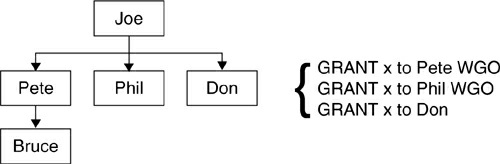
\includegraphics[width=0.6\textwidth]{figures/cascading_revokes}
    \begin{itemize}
        \item When a revoke causes the DBMS to revoke additional related privileges.
        \item Example: Joe grants privilege X to Pete and Phil (with GRANT option), Pete grants X to Bruce, Joe grants X to Don (without GRANT option).
        \item If X is revoked from Joe, it will also be revoked from Pete, Phil, Don, and Bruce (cascading effect).
        \item To minimize impact, avoid granting privileges using the WITH GRANT OPTION.
        \item Some DBMS products allow revoking without cascading.
    \end{itemize}
\end{frame}

\begin{frame}{Chronology and Revokes}
    \begin{itemize}
        \item Timing of GRANT or REVOKE can affect impact.
        \item Example: Grant DELETE on titles to public; COMMIT; REVOKE DELETE on titles from userx;
        \item In some DBMSs (e.g., Microsoft SQL Server), this sequence bars userx from deleting, even though PUBLIC was granted DELETE.
        \item Some DBMSs (e.g., DB2) do not permit such exclusions; PUBLIC overrides revokes.
        \item DBA must understand how GRANTs and REVOKEs work for each DBMS.
    \end{itemize}
\end{frame}

\begin{frame}{Label-Based Access Control (LBAC)}
    \begin{itemize}
        \item Need for low-level access control is critical as systems become more sophisticated.
        \item LBAC secures each piece of data, ensuring only authorized users can perform authorized functions.
        \item Supports applications needing a more granular security scheme.
        \item Can specify who can read and modify data in individual rows and/or columns.
    \end{itemize}
\end{frame}

\begin{frame}{LBAC Details}
    \begin{itemize}
        \item Administrator configures LBAC by creating security label components.
        \item Security policy, composed of label components, describes criteria for data access.
        \item Security administrator defines policy by creating security labels.
        \item Security label can be associated with columns and rows to protect data.
        \item Users are granted access by granting them security labels.
    \end{itemize}
\end{frame}

\begin{frame}{LBAC Process}
    \begin{itemize}
        \item When a user tries to access protected data, their security label is compared to the label protecting the data.
        \item Protecting label blocks some security labels but not others.
        \item Users can hold labels for multiple policies but at most one label for read and one for write access per policy.
        \item Exemptions can be granted to users, allowing access to data their labels might otherwise prevent.
        \item Security labels and exemptions are called LBAC credentials.
    \end{itemize}
\end{frame}

\begin{frame}{LBAC Implementation}
    \begin{itemize}
        \item Attempted access to a protected column fails if LBAC credentials do not permit it.
        \item If users try to read protected rows not allowed by their credentials, the DBMS acts as if those rows do not exist.
        \item Aggregate functions (e.g., COUNT(*)) ignore rows when LBAC credentials do not allow read access.
        \item Requires adding a specially named column to act as the security label.
        \item Security label column is matched with the multilevel security hierarchy set up by the administrator.
    \end{itemize}
\end{frame}

\begin{frame}{LBAC Hierarchy Example}
    \centering
    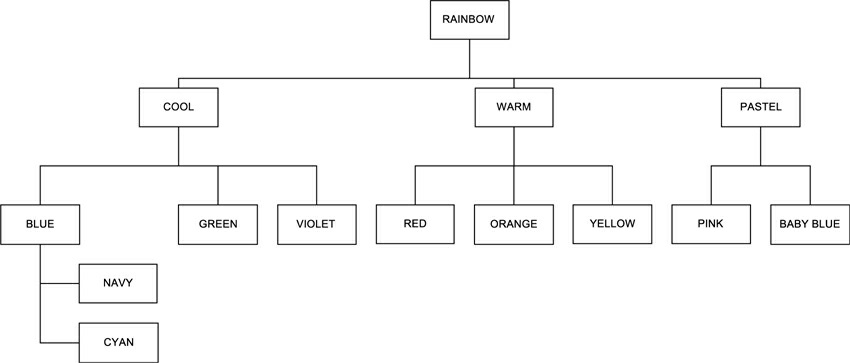
\includegraphics[width=0.9\textwidth]{figures/lbac}
    \begin{itemize}
        \item Hierarchy example uses colors (RAINBOW, COOL, WARM, PASTEL, BLUE, GREEN, VIOLET, NAVY, CYAN).
        \item Hierarchy need not be complex (e.g., TOP SECRET, SECRET, UNCLASSIFIED).
    \end{itemize}
\end{frame}
\begin{frame}{LBAC Hierarchy Example}
    \centering
    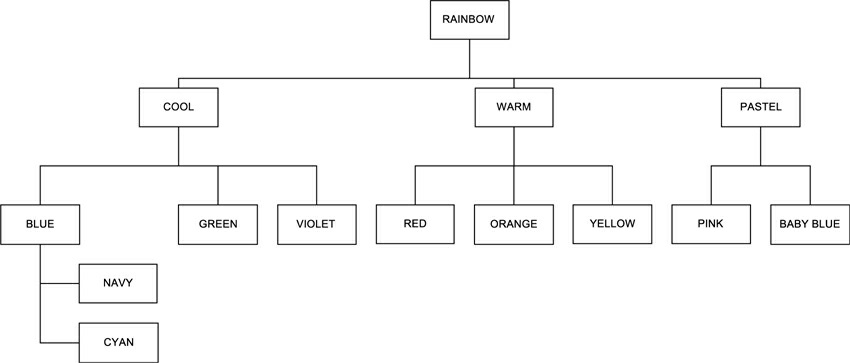
\includegraphics[width=0.9\textwidth]{figures/lbac}
    \begin{itemize}
        \item Hierarchy is established in security software (e.g., RACF with DB2 for z/OS).
        \item RAINBOW label includes everything.
        \item Middle levels (e.g., COOL, WARM, PASTEL) represent additional groupings.
    \end{itemize}
\end{frame}

\begin{frame}{LBAC Flexibility and Control}
    \begin{itemize}
        \item Hierarchy provides flexibility for assigning various security levels to data.
        \item Assigning a security label column and populating it controls whether a user can access a particular row.
        \item RAINBOW makes data accessible to anyone.
        \item NAVY is more restrictive.
        \item BLUE data can access BLUE rows and subordinate blue shades (NAVY and CYAN).
    \end{itemize}
\end{frame}

\begin{frame}{Security Reporting}
    \begin{itemize}
        \item DBA needs to monitor and report on user privileges.
        \item Database security is maintained in the system catalog.
        \item SQL can be used to retrieve information from system catalog tables.
        \item Some DBMSs provide views and system-stored procedures for easier retrieval.
        \item Protect the security of the system catalog, especially in production.
    \end{itemize}
\end{frame}

\begin{frame}{Security Reviews}
    \begin{itemize}
        \item User security requirements evolve over time.
        \item Database security needs to change as new applications are added and business requirements change.
        \item Regular security reviews are necessary to ensure implemented security matches current requirements.
        \item Reports from system catalog tables can provide input for reviews.
    \end{itemize}
\end{frame}

\begin{frame}{Authorization Roles and Groups}
    \begin{itemize}
        \item DBMS may allow assigning users specific privileges to a role or built-in groups of privileges.
        \item Terminology varies among DBMSs (roles vs. groups).
        \item DBA needs to understand how each DBMS implements roles and groups to simplify security administration.
    \end{itemize}
\end{frame}

\begin{frame}[fragile]{Roles}
    \begin{itemize}
        \item Role: Collection of privileges.
        \item DBA creates a role and assigns privileges to it.
        \item Role can be assigned to one or more users, simplifying security administration.
        \item Example:
            {\scriptsize
                \begin{verbatim}
CREATE role MANAGER; COMMIT;
GRANT select, insert, update, delete on employee to MANAGER;
GRANT select, insert, update, delete on job_title to MANAGER;
GRANT execute on payroll to MANAGER; COMMIT;
GRANT MANAGER to user1; COMMIT;
                \end{verbatim}
            }
        \item Additional users can be assigned the \texttt{MANAGER} role without needing to issue individual \texttt{GRANT} statements.
    \end{itemize}
\end{frame}

\begin{frame}{Groups}
    \begin{itemize}
        \item Group-level authority is similar to roles.
        \item DBMS provides built-in groups that cannot be changed.
        \item Each DBMS implements group-level security differently with different group names and privileges.
        \item Similarities exist across DBMSs.
    \end{itemize}
\end{frame}

\begin{frame}{Common Groups}
    \begin{itemize}
        \item System administrator (SA or SYSADM): Most powerful, can execute all commands and access all objects.
        \item Database administrator (DBADM or DBA): All privileges over a specific database, can access but not modify data.
        \item Database maintenance (DBMAINT): Privileges for maintaining database objects (e.g., utilities and commands).
        \item Security administrator: Privileges for granting/revoking security, login/password administration, auditing, security configuration.
        \item Operations control (OPER or SYSOPR): Authority to perform operational tasks like backup/recovery and terminating tasks.
    \end{itemize}
\end{frame}

\begin{frame}{Group Management}
    \begin{itemize}
        \item Limit the number of users with SA role or group-level authority.
        \item SA capabilities are very powerful; only corporate DBAs and systems programmers should have this authority.
        \item Group-Level Security and Cascading REVOKEs:
        \begin{itemize}
            \item Some group-level privileges allow users to grant privileges to others.
            \item Revoking group-level authority from such a user also revokes any privileges they granted.
            \item Similar to cascading REVOKEs with the WITH GRANT option.
        \end{itemize}
    \end{itemize}
\end{frame}

\begin{frame}{Using Views for Security}
    \begin{itemize}
        \item Views can simplify some aspects of database security.
        \item Example: Employee table with sensitive information (salary, etc.).
        \item Granting SELECT privilege on the table can cause a security problem.
        \item A view can be created to omit sensitive information.
        \item Users can be granted SELECT on the view to access appropriate information.
    \end{itemize}
\end{frame}

\begin{frame}[fragile]{Vertical Restriction with Views}
    \begin{itemize}
        \item Example View:
        {\scriptsize
        \begin{verbatim}
CREATE VIEW emp_all AS
SELECT
    first_name, last_name, middle_initial,
    street_address, state, zip_code
FROM
    employee;
        \end{verbatim}
        }
        \item Only information specified in the view can be retrieved.
        \item Eliminating columns from a base table to create a view is vertical restriction.
        \item Definition of sensitive data varies by organization.
    \end{itemize}
\end{frame}

\section{Using Stored Procedures for Security}

\begin{frame}{Stored Procedures for Security}
    \begin{itemize}
        \item Stored procedures enhance security by restricting direct access to base tables.
        \item Execution privilege must be explicitly granted or revoked.
        \item Ensures controlled data access through procedural logic.
    \end{itemize}
\end{frame}

\begin{frame}{Logic-Oriented Security}
    \begin{itemize}
        \item Implement security based on conditions such as user identity and time of access.
        \item Prevent unauthorized data manipulation.
        \item Example: Restrict access to specific hours.
    \end{itemize}
\end{frame}

\section{Encryption}

\begin{frame}{Encryption Overview}
    \begin{itemize}
        \item Protects data by transforming it into unreadable formats without decryption keys.
        \item Two primary types: \textbf{Data at Rest} and \textbf{Data in Transit} encryption.
        \item Used to comply with security regulations and prevent unauthorized access.
    \end{itemize}
\end{frame}

\begin{frame}{Encryption and Decryption}
    \centering
    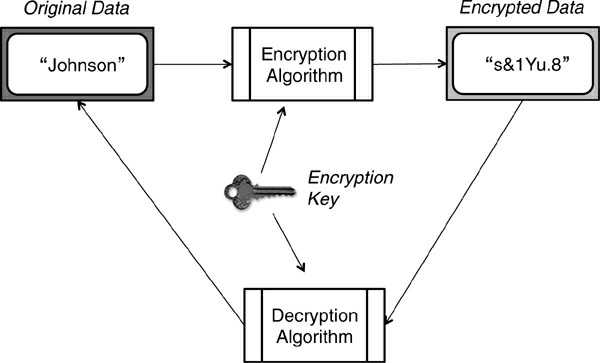
\includegraphics[width=0.75\textwidth]{figures/encryption}
\end{frame}

\begin{frame}{Types of Encryption}
    \begin{itemize}
        \item Data at Rest: Protects stored data from unauthorized access.
        \item Data in Transit: Ensures secure data transfer over networks.
        \item Common encryption techniques: AES, DES, and SHA hashing.
    \end{itemize}
\end{frame}

\section{SQL Injection}

\begin{frame}{SQL Injection Attacks}
    \begin{itemize}
        \item A technique used by attackers to execute unauthorized SQL commands.
        \item Exploits improper input validation in web applications.
        \item Can lead to data leaks, unauthorized modifications, or even database destruction.
    \end{itemize}
\end{frame}

\begin{frame}{Preventing SQL Injection}
    \begin{itemize}
        \item Validate all user inputs.
        \item Use prepared statements and parameterized queries.
        \item Restrict database permissions to limit exposure.
        \item Avoid concatenating user input in SQL statements.
    \end{itemize}
\end{frame}

\begin{frame}{Examples of SQL Injection Attacks}
    \begin{itemize}
        \item In 2006, Russian hackers stole credit card data from a Rhode Island government website.
        \item In 2007, a hacker defaced Microsoft's UK website using SQL injection.
        \item In 2008, tens of thousands of PCs were infected via an automated SQL injection attack targeting Microsoft SQL Server.
    \end{itemize}
\end{frame}

\begin{frame}{More SQL Injection Cases}
    \begin{itemize}
        \item In 2010, a Swedish voter attempted an SQL injection attack in a write-in vote.
        \item In 2011, the Public Broadcasting System (PBS) was hacked using SQL injection.
        \item Other victims: Barracuda Networks, MySQL.com, Lady Gaga’s website, Nokia, and Canon.
    \end{itemize}
\end{frame}

\section{Auditing}

\begin{frame}{Database Auditing}
    \begin{itemize}
        \item Tracks database activities to detect unauthorized access.
        \item Helps ensure compliance with security policies.
        \item Logs who accessed data, what was changed, and when.
    \end{itemize}
\end{frame}

\begin{frame}{Threats to Security}
    \begin{itemize}
        \item Internal threats from disgruntled employees.
        \item External cyber-attacks targeting sensitive information.
        \item Auditing helps in identifying and mitigating such threats.
    \end{itemize}
\end{frame}

\section{External Security}

\begin{frame}{External Security Mechanisms}
    \begin{itemize}
        \item Protect database files at the operating system level.
        \item Use firewalls, access controls, and encryption.
        \item Prevent unauthorized access outside DBMS control.
    \end{itemize}
\end{frame}

\section{Conclusion}

\begin{frame}{Summary}
    \begin{itemize}
        \item Database security is critical to protect sensitive data.
        \item Use stored procedures, encryption, and auditing to enhance security.
        \item Prevent SQL injection and secure external resources.
    \end{itemize}
\end{frame}

\begin{frame}{Database Administration: Database Security.}
    \centering
    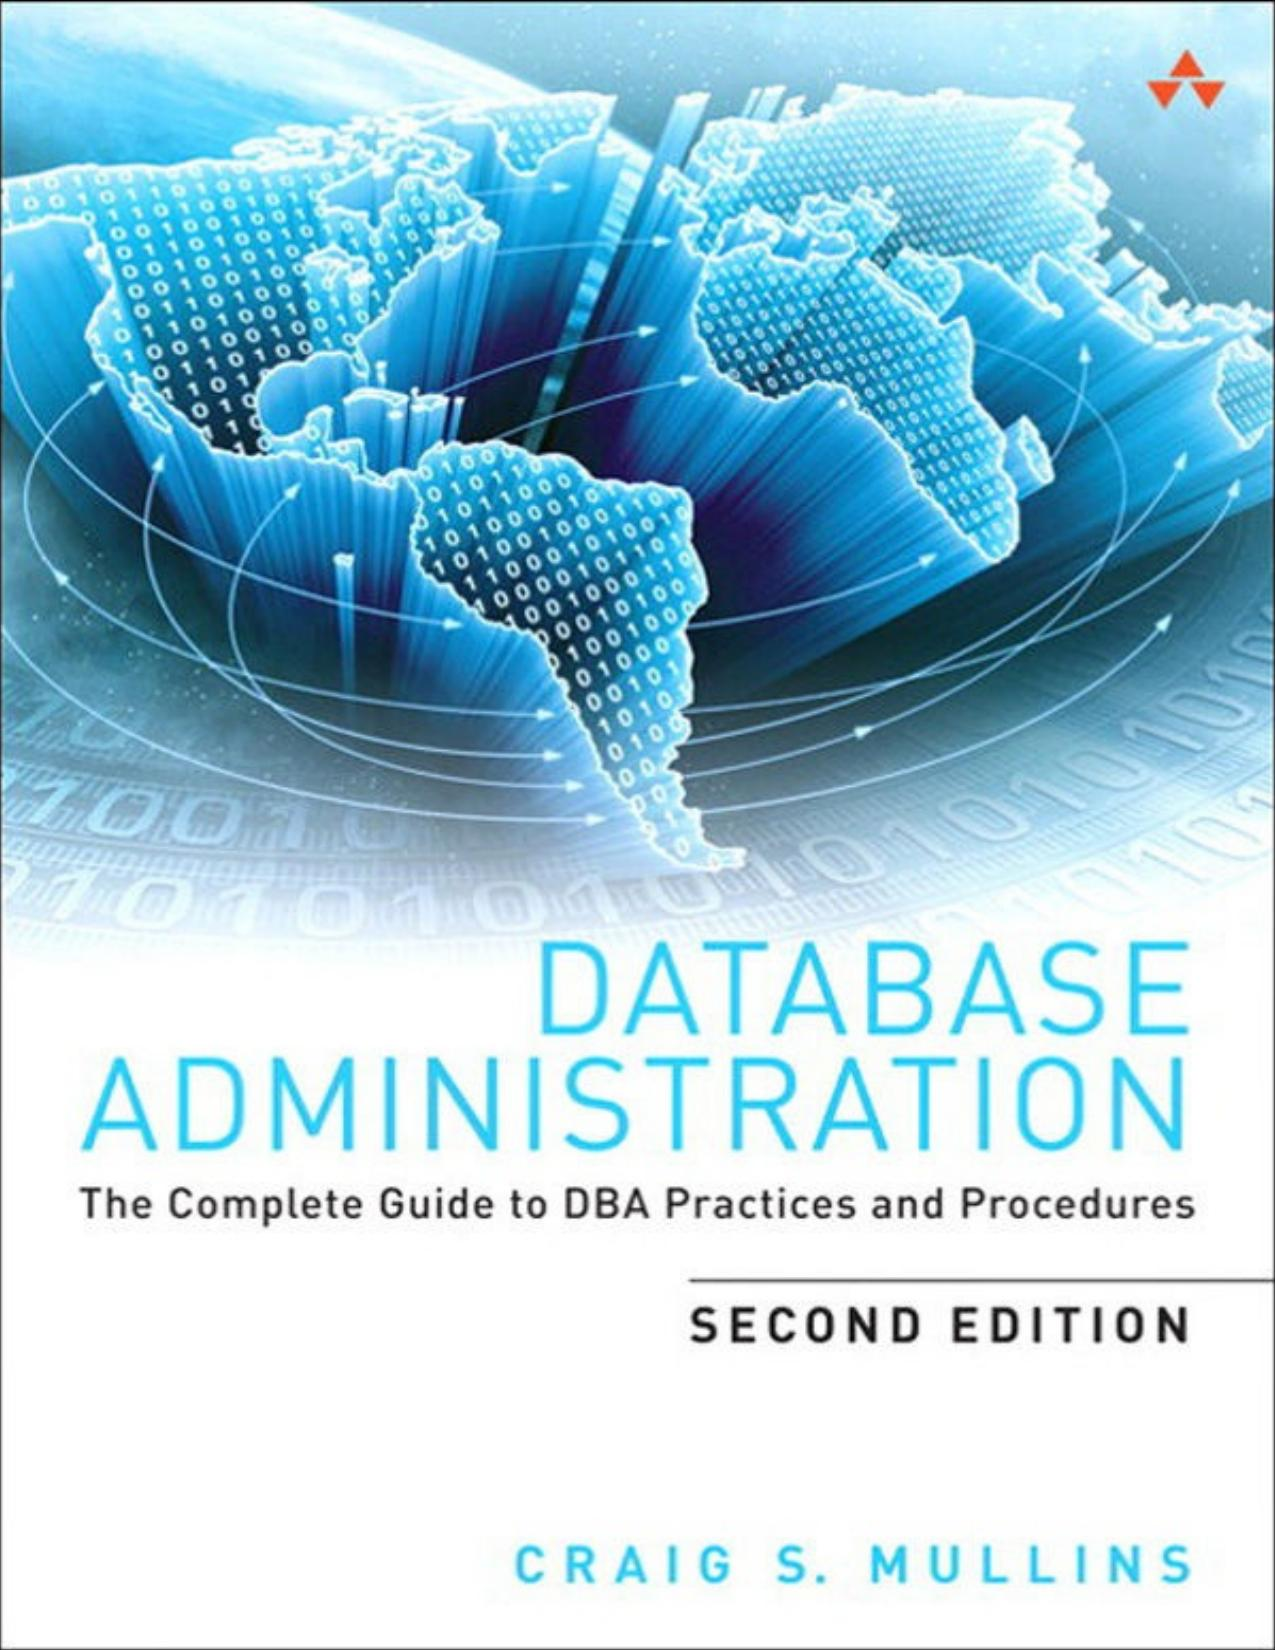
\includegraphics[width=0.4\textwidth]{figures/book_cover}\\
    \vspace{2mm}
    {
        \scriptsize
        Content has been extracted from \textit{Database Administration: The Complete Guide to DBA Practices and Procedure (Chapter 14)}, by Craig Mullins, 2013.  Visit \url{https://www.oreilly.com/library/view/database-administration-the/9780133012743/}.\\
    }
\end{frame}

\end{document}
